% Options for packages loaded elsewhere
\PassOptionsToPackage{unicode}{hyperref}
\PassOptionsToPackage{hyphens}{url}
%
\documentclass[
]{article}
\usepackage{amsmath,amssymb}
\usepackage{iftex}
\ifPDFTeX
  \usepackage[T1]{fontenc}
  \usepackage[utf8]{inputenc}
  \usepackage{textcomp} % provide euro and other symbols
\else % if luatex or xetex
  \usepackage{unicode-math} % this also loads fontspec
  \defaultfontfeatures{Scale=MatchLowercase}
  \defaultfontfeatures[\rmfamily]{Ligatures=TeX,Scale=1}
\fi
\usepackage{lmodern}
\ifPDFTeX\else
  % xetex/luatex font selection
\fi
% Use upquote if available, for straight quotes in verbatim environments
\IfFileExists{upquote.sty}{\usepackage{upquote}}{}
\IfFileExists{microtype.sty}{% use microtype if available
  \usepackage[]{microtype}
  \UseMicrotypeSet[protrusion]{basicmath} % disable protrusion for tt fonts
}{}
\makeatletter
\@ifundefined{KOMAClassName}{% if non-KOMA class
  \IfFileExists{parskip.sty}{%
    \usepackage{parskip}
  }{% else
    \setlength{\parindent}{0pt}
    \setlength{\parskip}{6pt plus 2pt minus 1pt}}
}{% if KOMA class
  \KOMAoptions{parskip=half}}
\makeatother
\usepackage{xcolor}
\usepackage[margin=1in]{geometry}
\usepackage{color}
\usepackage{fancyvrb}
\newcommand{\VerbBar}{|}
\newcommand{\VERB}{\Verb[commandchars=\\\{\}]}
\DefineVerbatimEnvironment{Highlighting}{Verbatim}{commandchars=\\\{\}}
% Add ',fontsize=\small' for more characters per line
\usepackage{framed}
\definecolor{shadecolor}{RGB}{248,248,248}
\newenvironment{Shaded}{\begin{snugshade}}{\end{snugshade}}
\newcommand{\AlertTok}[1]{\textcolor[rgb]{0.94,0.16,0.16}{#1}}
\newcommand{\AnnotationTok}[1]{\textcolor[rgb]{0.56,0.35,0.01}{\textbf{\textit{#1}}}}
\newcommand{\AttributeTok}[1]{\textcolor[rgb]{0.13,0.29,0.53}{#1}}
\newcommand{\BaseNTok}[1]{\textcolor[rgb]{0.00,0.00,0.81}{#1}}
\newcommand{\BuiltInTok}[1]{#1}
\newcommand{\CharTok}[1]{\textcolor[rgb]{0.31,0.60,0.02}{#1}}
\newcommand{\CommentTok}[1]{\textcolor[rgb]{0.56,0.35,0.01}{\textit{#1}}}
\newcommand{\CommentVarTok}[1]{\textcolor[rgb]{0.56,0.35,0.01}{\textbf{\textit{#1}}}}
\newcommand{\ConstantTok}[1]{\textcolor[rgb]{0.56,0.35,0.01}{#1}}
\newcommand{\ControlFlowTok}[1]{\textcolor[rgb]{0.13,0.29,0.53}{\textbf{#1}}}
\newcommand{\DataTypeTok}[1]{\textcolor[rgb]{0.13,0.29,0.53}{#1}}
\newcommand{\DecValTok}[1]{\textcolor[rgb]{0.00,0.00,0.81}{#1}}
\newcommand{\DocumentationTok}[1]{\textcolor[rgb]{0.56,0.35,0.01}{\textbf{\textit{#1}}}}
\newcommand{\ErrorTok}[1]{\textcolor[rgb]{0.64,0.00,0.00}{\textbf{#1}}}
\newcommand{\ExtensionTok}[1]{#1}
\newcommand{\FloatTok}[1]{\textcolor[rgb]{0.00,0.00,0.81}{#1}}
\newcommand{\FunctionTok}[1]{\textcolor[rgb]{0.13,0.29,0.53}{\textbf{#1}}}
\newcommand{\ImportTok}[1]{#1}
\newcommand{\InformationTok}[1]{\textcolor[rgb]{0.56,0.35,0.01}{\textbf{\textit{#1}}}}
\newcommand{\KeywordTok}[1]{\textcolor[rgb]{0.13,0.29,0.53}{\textbf{#1}}}
\newcommand{\NormalTok}[1]{#1}
\newcommand{\OperatorTok}[1]{\textcolor[rgb]{0.81,0.36,0.00}{\textbf{#1}}}
\newcommand{\OtherTok}[1]{\textcolor[rgb]{0.56,0.35,0.01}{#1}}
\newcommand{\PreprocessorTok}[1]{\textcolor[rgb]{0.56,0.35,0.01}{\textit{#1}}}
\newcommand{\RegionMarkerTok}[1]{#1}
\newcommand{\SpecialCharTok}[1]{\textcolor[rgb]{0.81,0.36,0.00}{\textbf{#1}}}
\newcommand{\SpecialStringTok}[1]{\textcolor[rgb]{0.31,0.60,0.02}{#1}}
\newcommand{\StringTok}[1]{\textcolor[rgb]{0.31,0.60,0.02}{#1}}
\newcommand{\VariableTok}[1]{\textcolor[rgb]{0.00,0.00,0.00}{#1}}
\newcommand{\VerbatimStringTok}[1]{\textcolor[rgb]{0.31,0.60,0.02}{#1}}
\newcommand{\WarningTok}[1]{\textcolor[rgb]{0.56,0.35,0.01}{\textbf{\textit{#1}}}}
\usepackage{longtable,booktabs,array}
\usepackage{calc} % for calculating minipage widths
% Correct order of tables after \paragraph or \subparagraph
\usepackage{etoolbox}
\makeatletter
\patchcmd\longtable{\par}{\if@noskipsec\mbox{}\fi\par}{}{}
\makeatother
% Allow footnotes in longtable head/foot
\IfFileExists{footnotehyper.sty}{\usepackage{footnotehyper}}{\usepackage{footnote}}
\makesavenoteenv{longtable}
\usepackage{graphicx}
\makeatletter
\def\maxwidth{\ifdim\Gin@nat@width>\linewidth\linewidth\else\Gin@nat@width\fi}
\def\maxheight{\ifdim\Gin@nat@height>\textheight\textheight\else\Gin@nat@height\fi}
\makeatother
% Scale images if necessary, so that they will not overflow the page
% margins by default, and it is still possible to overwrite the defaults
% using explicit options in \includegraphics[width, height, ...]{}
\setkeys{Gin}{width=\maxwidth,height=\maxheight,keepaspectratio}
% Set default figure placement to htbp
\makeatletter
\def\fps@figure{htbp}
\makeatother
\setlength{\emergencystretch}{3em} % prevent overfull lines
\providecommand{\tightlist}{%
  \setlength{\itemsep}{0pt}\setlength{\parskip}{0pt}}
\setcounter{secnumdepth}{-\maxdimen} % remove section numbering
\usepackage{booktabs}
\usepackage{longtable}
\usepackage{array}
\usepackage{multirow}
\usepackage{wrapfig}
\usepackage{float}
\usepackage{colortbl}
\usepackage{pdflscape}
\usepackage{tabu}
\usepackage{threeparttable}
\usepackage{threeparttablex}
\usepackage[normalem]{ulem}
\usepackage{makecell}
\usepackage{xcolor}
\ifLuaTeX
  \usepackage{selnolig}  % disable illegal ligatures
\fi
\usepackage{bookmark}
\IfFileExists{xurl.sty}{\usepackage{xurl}}{} % add URL line breaks if available
\urlstyle{same}
\hypersetup{
  pdftitle={Methane Forecasting},
  hidelinks,
  pdfcreator={LaTeX via pandoc}}

\title{Methane Forecasting}
\author{}
\date{\vspace{-2.5em}}

\begin{document}
\maketitle

\section{Preparation}\label{preparation}

\subsection{Deseason Data}\label{deseason-data}

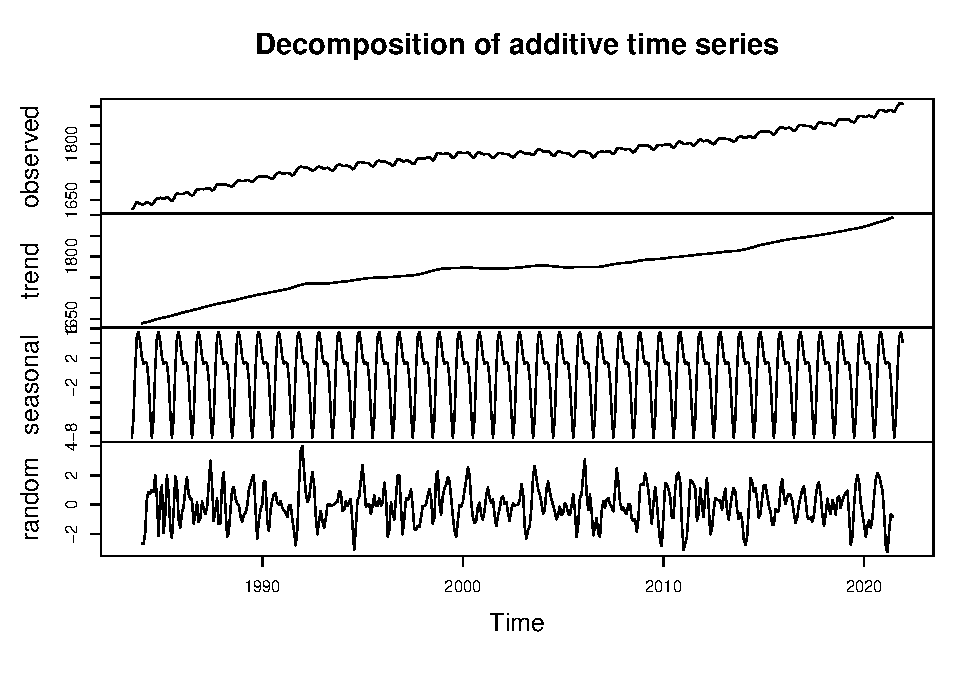
\includegraphics{Methane_Forecasting_files/figure-latex/unnamed-chunk-2-1.pdf}

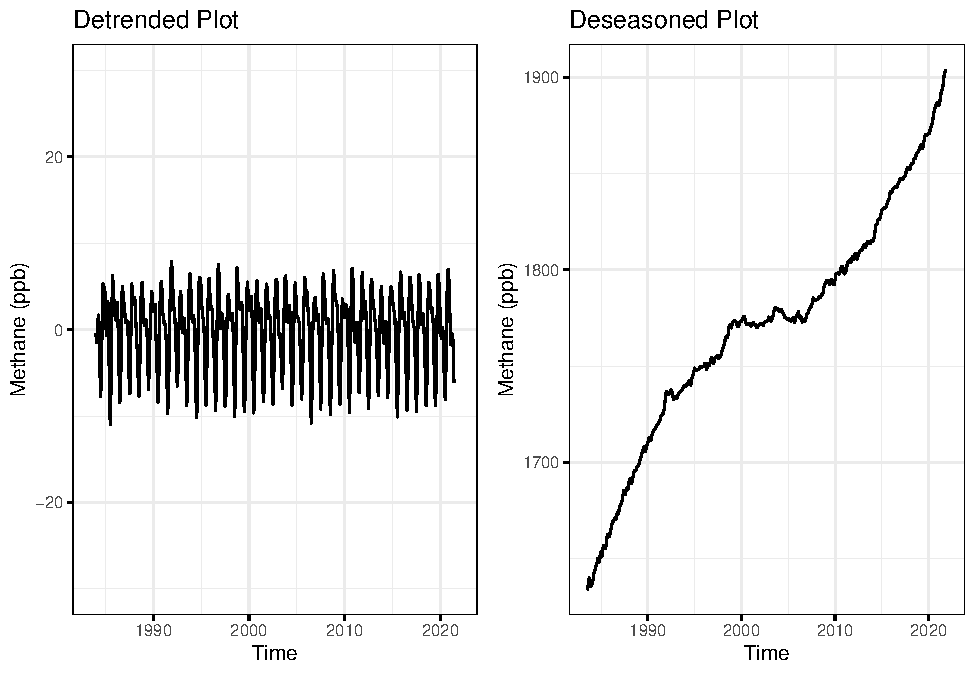
\includegraphics{Methane_Forecasting_files/figure-latex/unnamed-chunk-3-1.pdf}

\subsection{ACF and PACF}\label{acf-and-pacf}

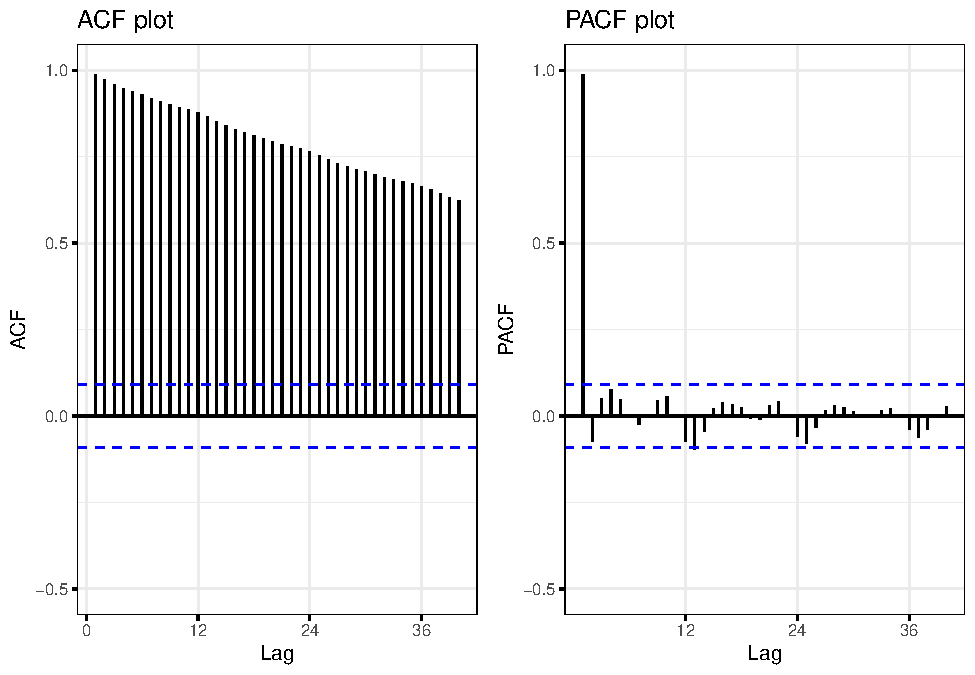
\includegraphics{Methane_Forecasting_files/figure-latex/unnamed-chunk-4-1.pdf}

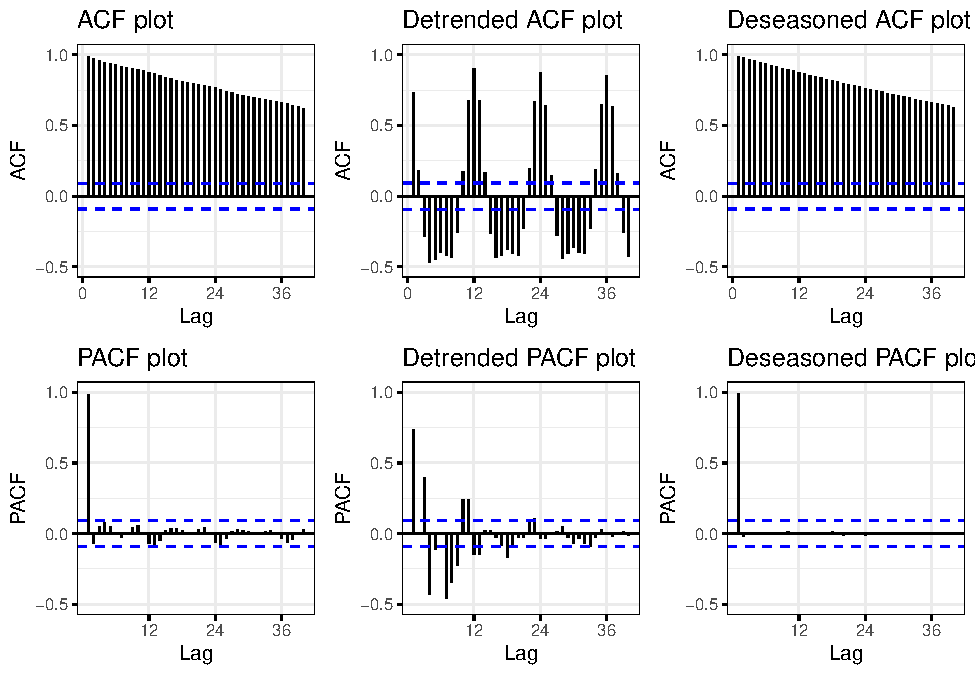
\includegraphics{Methane_Forecasting_files/figure-latex/unnamed-chunk-5-1.pdf}

\subsection{Stationarity Tests}\label{stationarity-tests}

\begin{verbatim}
## [1] "Results from Seasonal Mann-Kendall Test for orginal data"
\end{verbatim}

\begin{verbatim}
## Score =  8432 , Var(Score) = 78964
## denominator =  8664
## tau = 0.973, 2-sided pvalue =< 2.22e-16
\end{verbatim}

\begin{verbatim}
## [1] "Results from Mann-Kendall Test for deseasoned data"
\end{verbatim}

\begin{verbatim}
## Score =  102531 , Var(Score) = 10992237
## denominator =  106491
## tau = 0.963, 2-sided pvalue =< 2.22e-16
\end{verbatim}

\begin{verbatim}
## [1] "Results from ADF test for original data"
\end{verbatim}

\begin{verbatim}
## 
##  Augmented Dickey-Fuller Test
## 
## data:  methane_train_ts
## Dickey-Fuller = -1.5755, Lag order = 7, p-value = 0.7574
## alternative hypothesis: stationary
\end{verbatim}

\begin{verbatim}
## [1] "Results from Spearman Correlation"
\end{verbatim}

\begin{verbatim}
## 
##  Spearman's rank correlation rho
## 
## data:  methane_train_ts and c(1:462)
## S = 169160, p-value < 2.2e-16
## alternative hypothesis: true rho is not equal to 0
## sample estimates:
##       rho 
## 0.9897074
\end{verbatim}

\section{Forecasting Models}\label{forecasting-models}

\subsection{ARIMA}\label{arima}

\begin{verbatim}
## Series: methane_deseasoned 
## ARIMA(5,2,4) 
## 
## Coefficients:
##           ar1      ar2      ar3      ar4      ar5     ma1      ma2      ma3
##       -1.0263  -0.7132  -0.3662  -0.1259  -0.1462  1.3931  -0.4270  -1.3047
## s.e.   0.2188   0.1245   0.1203   0.0717   0.0555  0.2176   0.1859   0.1961
##           ma4
##       -0.4437
## s.e.   0.1835
## 
## sigma^2 = 0.431:  log likelihood = -451.77
## AIC=923.54   AICc=924.03   BIC=964.85
\end{verbatim}

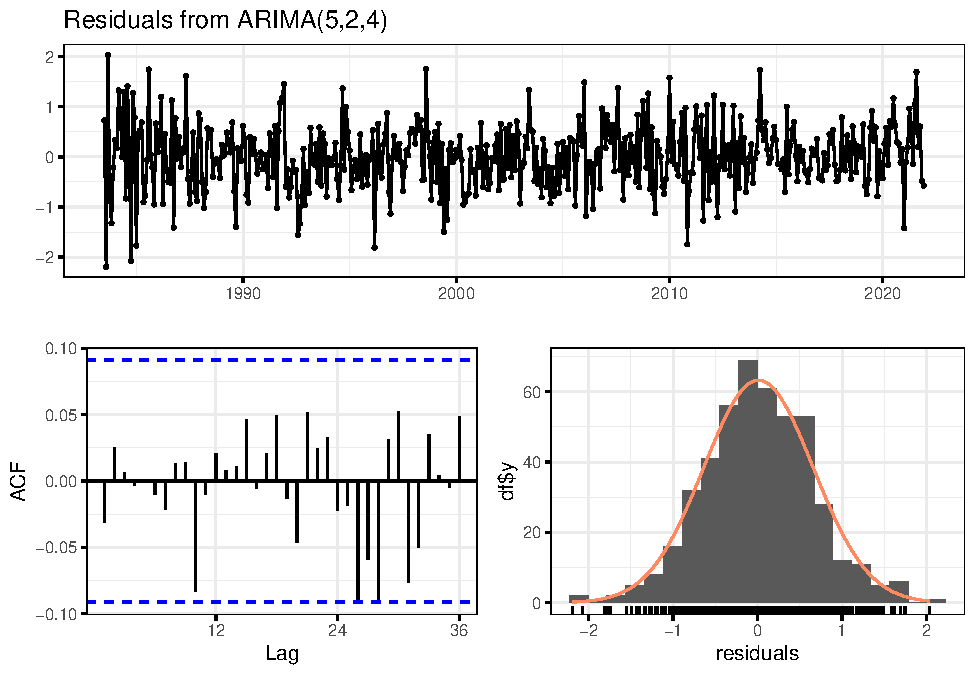
\includegraphics{Methane_Forecasting_files/figure-latex/unnamed-chunk-9-1.pdf}

\begin{verbatim}
## 
##  Ljung-Box test
## 
## data:  Residuals from ARIMA(5,2,4)
## Q* = 10.766, df = 15, p-value = 0.769
## 
## Model df: 9.   Total lags used: 24
\end{verbatim}

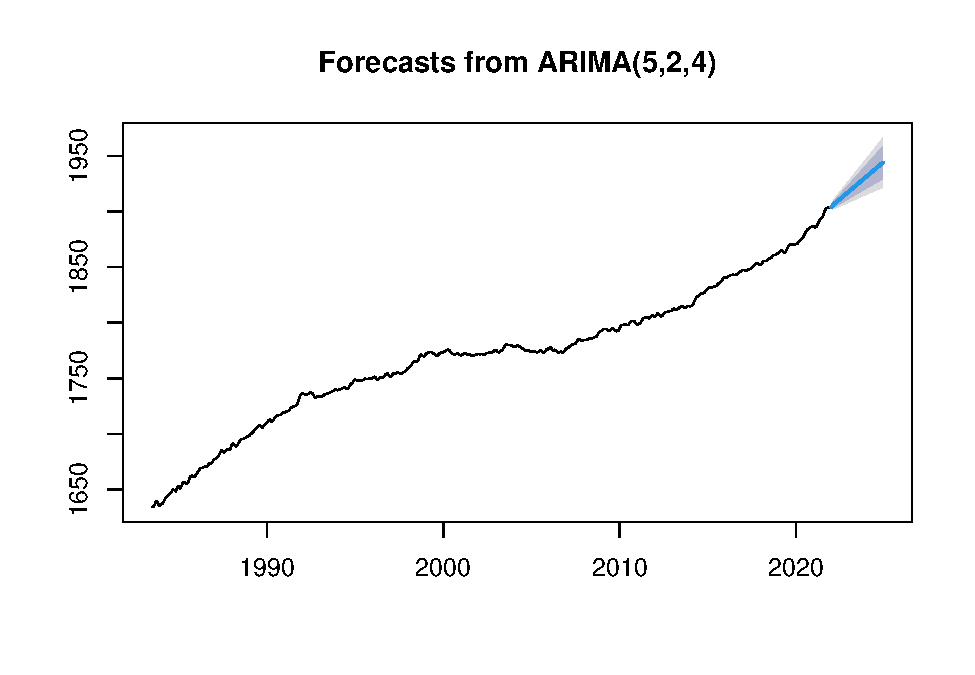
\includegraphics{Methane_Forecasting_files/figure-latex/unnamed-chunk-9-2.pdf}

The ARIMA auto-fit was: ARIMA(5,2,4).

The residuals look pretty good. Otherwise, the residuals are primarily
not significant in the ACF plot and are normally distributed.

\subsection{SARIMA}\label{sarima}

\begin{verbatim}
## Series: methane_train_ts 
## ARIMA(2,1,2)(1,1,1)[12] 
## 
## Coefficients:
##           ar1      ar2     ma1     ma2    sar1     sma1
##       -0.3875  -0.3977  1.7665  0.8226  0.0635  -0.8639
## s.e.   0.0504   0.0470  0.0353  0.0347  0.0740   0.0598
## 
## sigma^2 = 0.5296:  log likelihood = -465.66
## AIC=945.32   AICc=945.57   BIC=974.07
\end{verbatim}

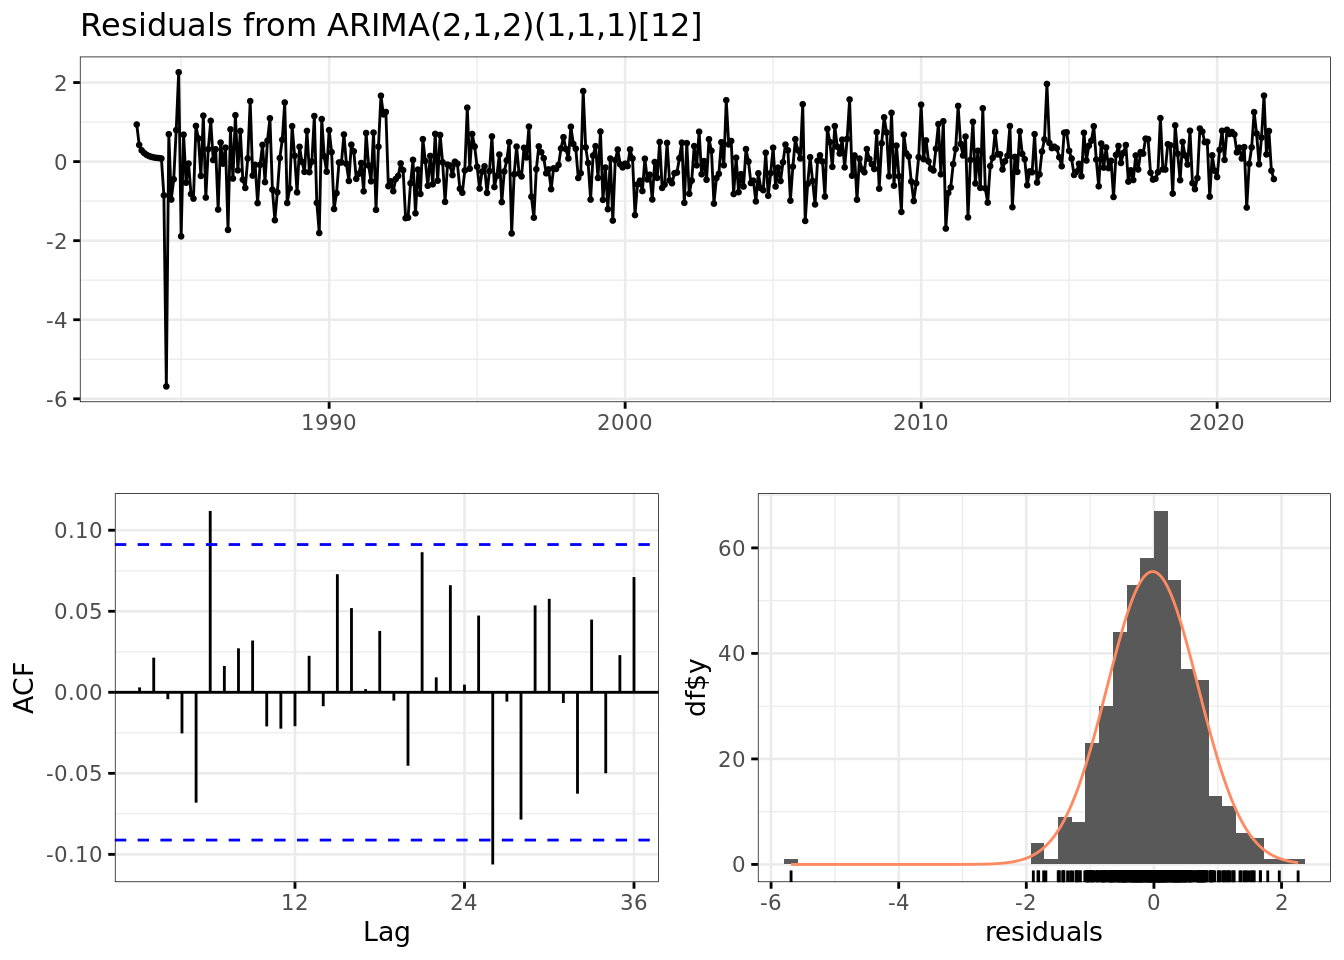
\includegraphics{Methane_Forecasting_files/figure-latex/unnamed-chunk-10-1.pdf}

\begin{verbatim}
## 
##  Ljung-Box test
## 
## data:  Residuals from ARIMA(2,1,2)(1,1,1)[12]
## Q* = 21.848, df = 18, p-value = 0.2388
## 
## Model df: 6.   Total lags used: 24
\end{verbatim}

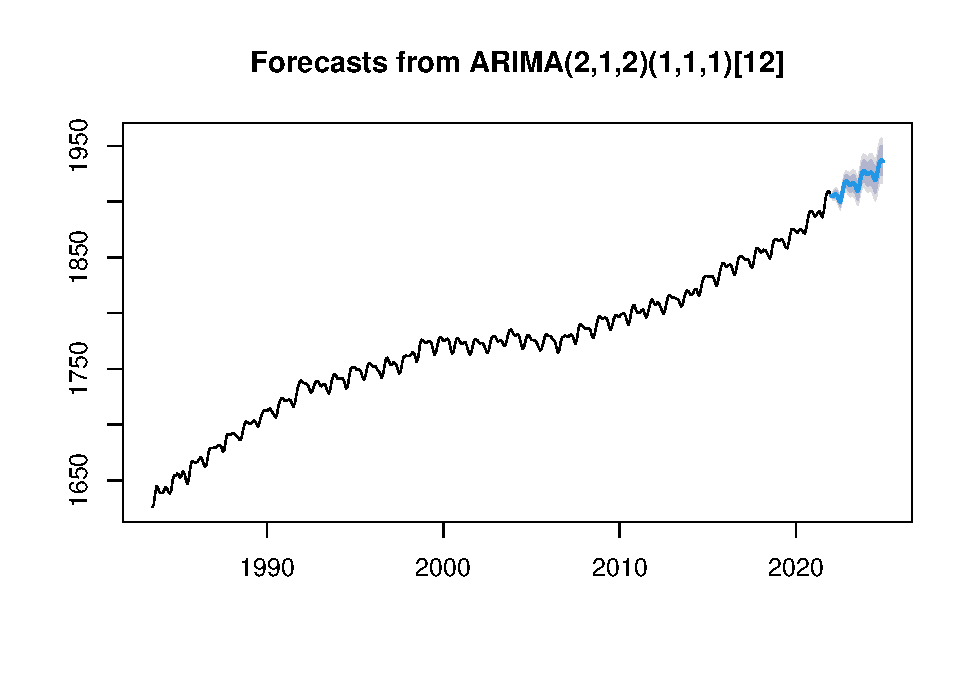
\includegraphics{Methane_Forecasting_files/figure-latex/unnamed-chunk-10-2.pdf}

The SARIMA auto-fit was: ARIMA(2,1,2)(1,1,1){[}12{]}.

The residuals look pretty good. There is one notable outlier. Otherwise,
the residuals are primarily not significant in the ACF plot and are
normally distributed.

\subsection{ARIMA with Fourier}\label{arima-with-fourier}

\begin{verbatim}
## Series: methane_train_msts 
## Regression with ARIMA(0,2,1) errors 
## Box Cox transformation: lambda= 0 
## 
## Coefficients:
##           ma1    S1-4   C1-4  C2-4   S1-12    C1-12    S2-12   C2-12  S4-12
##       -0.9659  -3e-04  2e-04     0  -6e-04  -0.0028  -0.0018  -5e-04      0
## s.e.   0.0113   1e-04  1e-04     0   1e-04   0.0002   0.0001   1e-04      0
##       C4-12  S5-12  C5-12
##       1e-04      0      0
## s.e.  0e+00      0      0
## 
## sigma^2 = 6.914e-07:  log likelihood = 2714.78
## AIC=-5403.56   AICc=-5402.74   BIC=-5349.85
\end{verbatim}

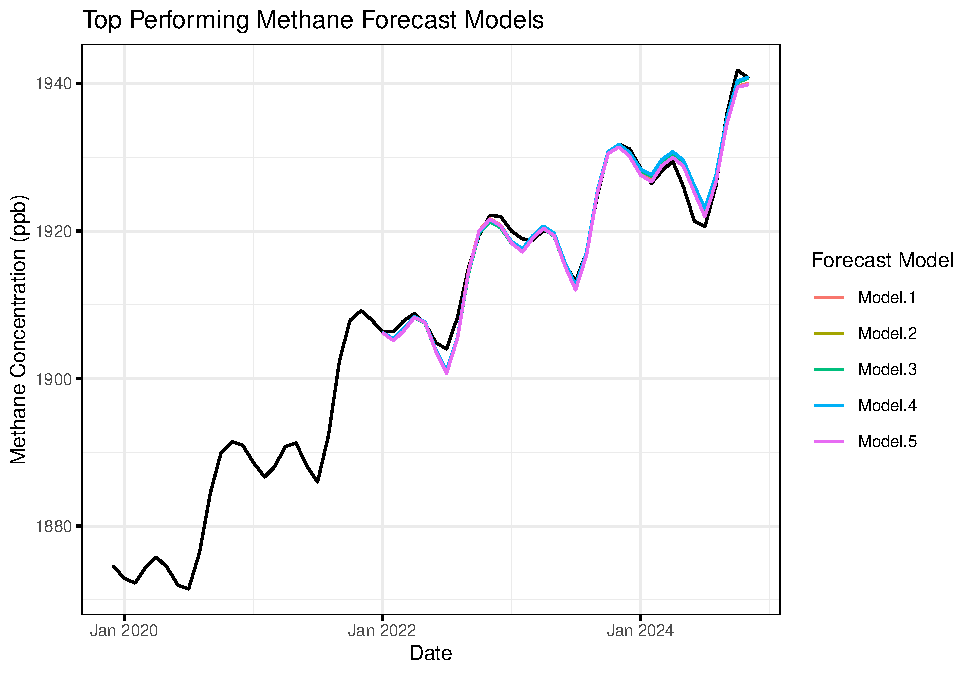
\includegraphics{Methane_Forecasting_files/figure-latex/unnamed-chunk-11-1.pdf}

\begin{verbatim}
## 
##  Ljung-Box test
## 
## data:  Residuals from Regression with ARIMA(0,2,1) errors
## Q* = 50.454, df = 23, p-value = 0.0008029
## 
## Model df: 1.   Total lags used: 24
\end{verbatim}

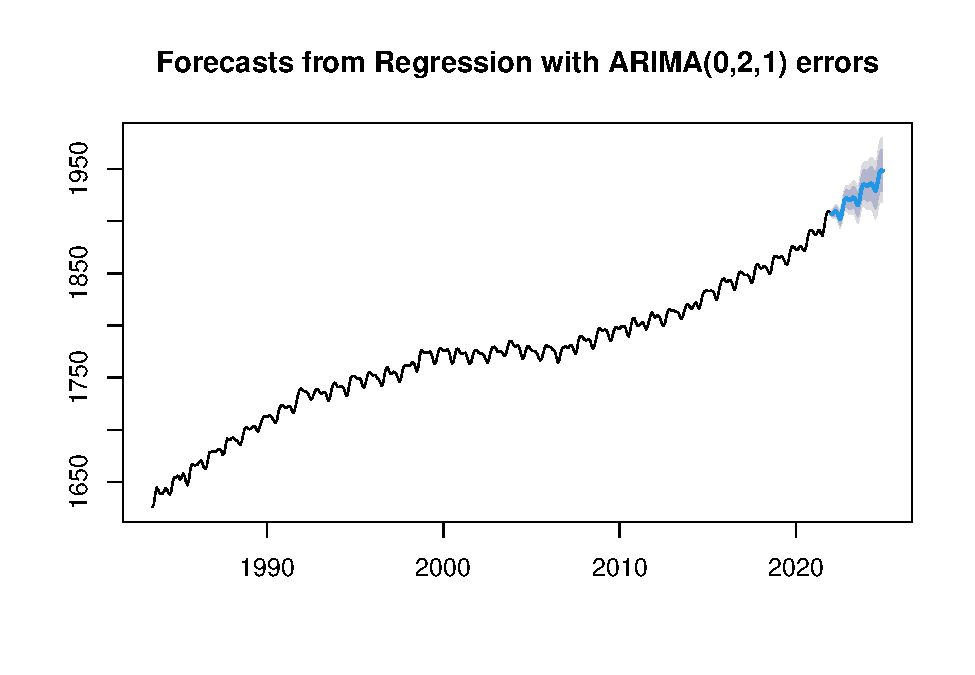
\includegraphics{Methane_Forecasting_files/figure-latex/unnamed-chunk-11-2.pdf}

\#\#STL+ETS

\begin{Shaded}
\begin{Highlighting}[]
\CommentTok{\#fit STL with ETS}
\NormalTok{stl\_ets\_fit }\OtherTok{\textless{}{-}} \FunctionTok{stlm}\NormalTok{(methane\_train\_ts, }\AttributeTok{s.window =} \StringTok{"periodic"}\NormalTok{, }\AttributeTok{method =} \StringTok{"ets"}\NormalTok{)}
\FunctionTok{print}\NormalTok{(stl\_ets\_fit}\SpecialCharTok{$}\NormalTok{model)}
\end{Highlighting}
\end{Shaded}

\begin{verbatim}
## ETS(A,A,N) 
## 
## Call:
## ets(y = x, model = etsmodel, allow.multiplicative.trend = allow.multiplicative.trend)
## 
##   Smoothing parameters:
##     alpha = 0.9999 
##     beta  = 0.0399 
## 
##   Initial states:
##     l = 1635.3113 
##     b = 0.4452 
## 
##   sigma:  1.1587
## 
##      AIC     AICc      BIC 
## 2976.741 2976.872 2997.419
\end{verbatim}

\begin{Shaded}
\begin{Highlighting}[]
\CommentTok{\#forecasting test data}
\NormalTok{stl\_ets\_forecast }\OtherTok{\textless{}{-}} \FunctionTok{forecast}\NormalTok{(stl\_ets\_fit, }\AttributeTok{h =} \FunctionTok{length}\NormalTok{(methane\_test\_ts))}

\CommentTok{\#accuracy assessment}
\NormalTok{stl\_ets\_accuracy }\OtherTok{\textless{}{-}} \FunctionTok{accuracy}\NormalTok{(stl\_ets\_forecast}\SpecialCharTok{$}\NormalTok{mean, methane\_test\_ts)}

\CommentTok{\#visualization}
\FunctionTok{plot}\NormalTok{(stl\_ets\_forecast)}
\end{Highlighting}
\end{Shaded}

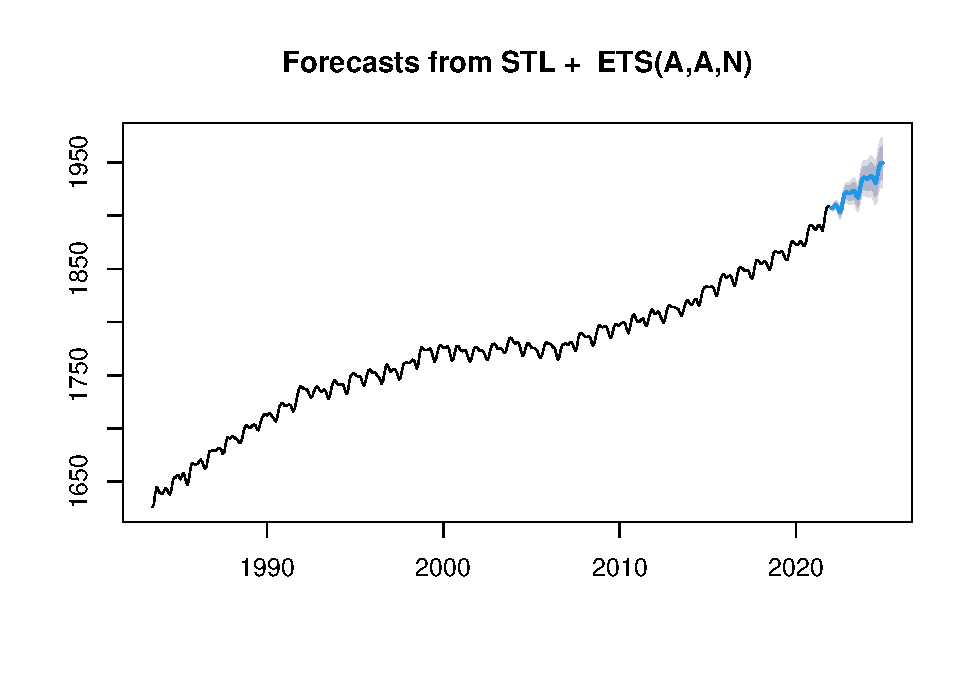
\includegraphics{Methane_Forecasting_files/figure-latex/unnamed-chunk-12-1.pdf}

\#\#TBATS

\begin{Shaded}
\begin{Highlighting}[]
\CommentTok{\#fit TBATS}
\NormalTok{tbats\_fit }\OtherTok{\textless{}{-}} \FunctionTok{tbats}\NormalTok{(methane\_train\_msts)}
\FunctionTok{print}\NormalTok{(tbats\_fit)}
\end{Highlighting}
\end{Shaded}

\begin{verbatim}
## TBATS(0.068, {2,2}, 1, {<4,1>, <12,2>})
## 
## Call: tbats(y = methane_train_msts)
## 
## Parameters
##   Lambda: 0.068322
##   Alpha: 1.739123
##   Beta: 0.03728037
##   Damping Parameter: 1
##   Gamma-1 Values: -0.0001741673 -0.001404042
##   Gamma-2 Values: -0.001057712 0.0001700574
##   AR coefficients: -0.950655 -0.850433
##   MA coefficients: 1.105508 0.740342
## 
## Seed States:
##                [,1]
##  [1,]  9.6256078766
##  [2,]  0.0009033680
##  [3,] -0.0005397463
##  [4,] -0.0002460857
##  [5,] -0.0042744805
##  [6,] -0.0028490611
##  [7,]  0.0014294959
##  [8,] -0.0008039491
##  [9,]  0.0000000000
## [10,]  0.0000000000
## [11,]  0.0000000000
## [12,]  0.0000000000
## attr(,"lambda")
## [1] 0.06832222
## 
## Sigma: 0.0008188126
## AIC: 2751.207
\end{verbatim}

\begin{Shaded}
\begin{Highlighting}[]
\FunctionTok{checkresiduals}\NormalTok{(tbats\_fit)}
\end{Highlighting}
\end{Shaded}

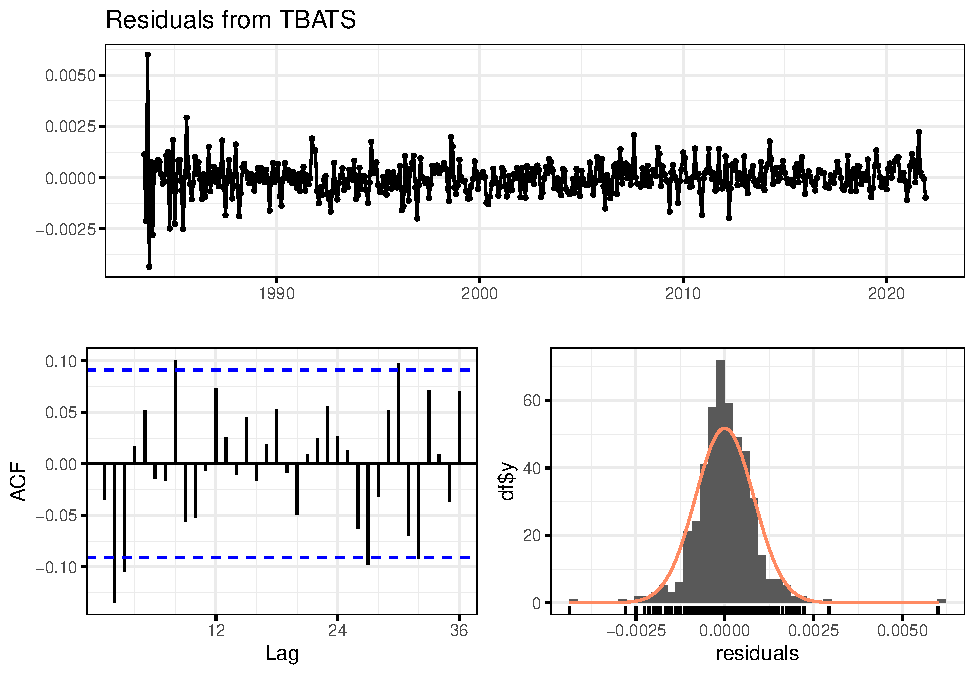
\includegraphics{Methane_Forecasting_files/figure-latex/unnamed-chunk-13-1.pdf}

\begin{verbatim}
## 
##  Ljung-Box test
## 
## data:  Residuals from TBATS
## Q* = 32.217, df = 24, p-value = 0.1217
## 
## Model df: 0.   Total lags used: 24
\end{verbatim}

\begin{Shaded}
\begin{Highlighting}[]
\CommentTok{\#forecasting test data}
\NormalTok{tbats\_forecast }\OtherTok{\textless{}{-}} \FunctionTok{forecast}\NormalTok{(tbats\_fit, }\AttributeTok{h =} \FunctionTok{length}\NormalTok{(methane\_test\_ts))}

\CommentTok{\#accuracy assessment}
\NormalTok{tbats\_accuracy }\OtherTok{\textless{}{-}} \FunctionTok{accuracy}\NormalTok{(tbats\_forecast}\SpecialCharTok{$}\NormalTok{mean, methane\_test\_ts)}

\CommentTok{\#visualization}
\FunctionTok{plot}\NormalTok{(tbats\_forecast)}
\end{Highlighting}
\end{Shaded}

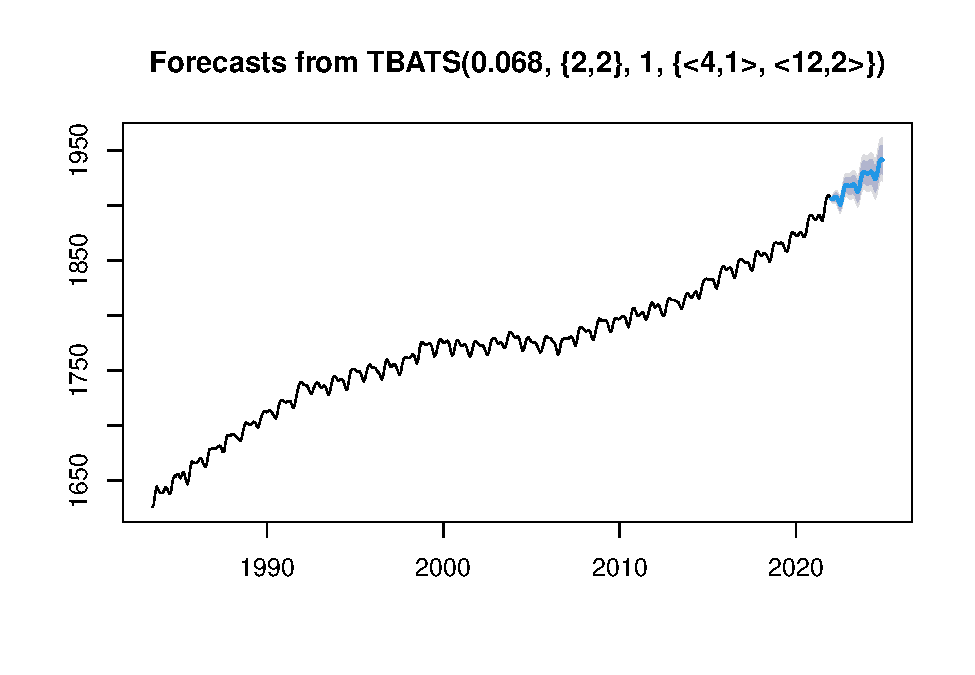
\includegraphics{Methane_Forecasting_files/figure-latex/unnamed-chunk-13-2.pdf}

\subsection{Neuron Network}\label{neuron-network}

\begin{Shaded}
\begin{Highlighting}[]
\NormalTok{NN\_fit }\OtherTok{\textless{}{-}} \FunctionTok{nnetar}\NormalTok{(methane\_train\_ts, }\AttributeTok{p =} \DecValTok{1}\NormalTok{, }\AttributeTok{P =} \DecValTok{7}\NormalTok{)}

\NormalTok{NN\_for }\OtherTok{\textless{}{-}} \FunctionTok{forecast}\NormalTok{(NN\_fit, }\AttributeTok{h=}\DecValTok{36}\NormalTok{)}

\NormalTok{forecast\_NN\_accuracy }\OtherTok{\textless{}{-}} \FunctionTok{accuracy}\NormalTok{(NN\_for}\SpecialCharTok{$}\NormalTok{mean, methane\_test\_ts)}

\FunctionTok{print}\NormalTok{(forecast\_NN\_accuracy)}
\end{Highlighting}
\end{Shaded}

\begin{verbatim}
##                ME     RMSE     MAE       MPE      MAPE      ACF1 Theil's U
## Test set 2.610708 3.624126 2.70236 0.1356465 0.1404314 0.7047191  1.001878
\end{verbatim}

\begin{Shaded}
\begin{Highlighting}[]
\FunctionTok{plot}\NormalTok{(NN\_for)}
\end{Highlighting}
\end{Shaded}

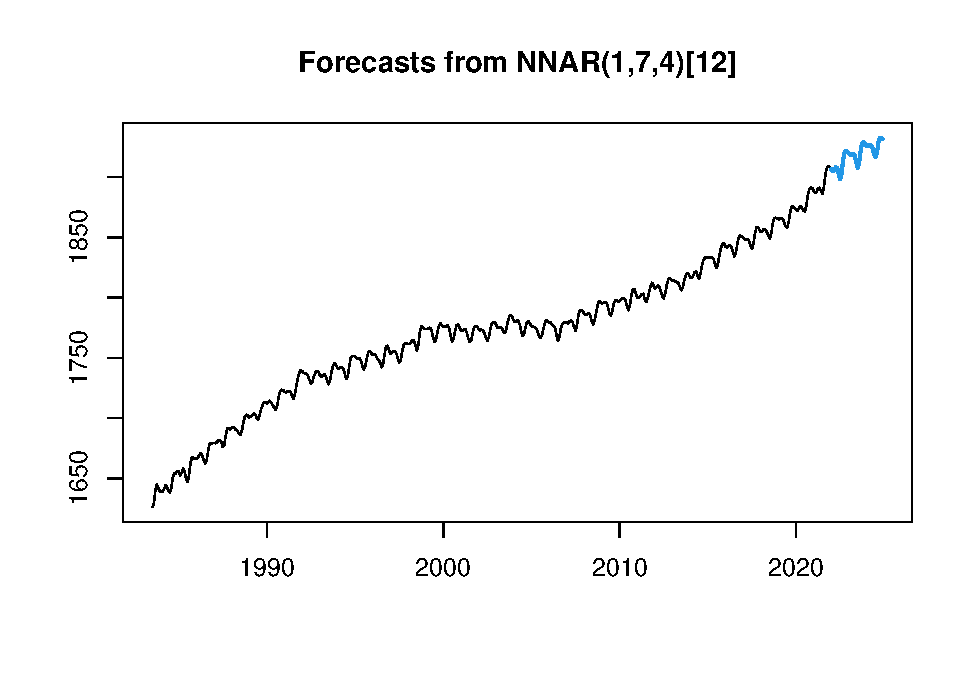
\includegraphics{Methane_Forecasting_files/figure-latex/unnamed-chunk-14-1.pdf}

\begin{Shaded}
\begin{Highlighting}[]
\NormalTok{NN\_fourier\_fit }\OtherTok{\textless{}{-}} \FunctionTok{nnetar}\NormalTok{(methane\_train\_msts, }\AttributeTok{p =} \DecValTok{0}\NormalTok{, }\AttributeTok{P =} \DecValTok{7}\NormalTok{,}
                 \AttributeTok{xreg=}\FunctionTok{fourier}\NormalTok{(methane\_train\_msts,}\AttributeTok{K=}\FunctionTok{c}\NormalTok{(}\DecValTok{2}\NormalTok{,}\DecValTok{6}\NormalTok{)))}

\NormalTok{NN\_fourier\_for }\OtherTok{\textless{}{-}} \FunctionTok{forecast}\NormalTok{(NN\_fourier\_fit, }\AttributeTok{h=}\DecValTok{36}\NormalTok{, }\AttributeTok{xreg=}\FunctionTok{fourier}\NormalTok{(methane\_train\_msts,}\AttributeTok{K=}\FunctionTok{c}\NormalTok{(}\DecValTok{2}\NormalTok{,}\DecValTok{6}\NormalTok{), }\AttributeTok{h=}\DecValTok{36}\NormalTok{))}

\NormalTok{forecast\_NN\_fourier\_accuracy }\OtherTok{\textless{}{-}} \FunctionTok{accuracy}\NormalTok{(NN\_fourier\_for}\SpecialCharTok{$}\NormalTok{mean, methane\_test\_msts)}

\FunctionTok{print}\NormalTok{(forecast\_NN\_fourier\_accuracy)}
\end{Highlighting}
\end{Shaded}

\begin{verbatim}
##                ME     RMSE      MAE       MPE      MAPE      ACF1 Theil's U
## Test set 7.041148 8.063206 7.046965 0.3663598 0.3666629 0.6777405  2.221493
\end{verbatim}

\begin{Shaded}
\begin{Highlighting}[]
\FunctionTok{plot}\NormalTok{(NN\_fourier\_for)}
\end{Highlighting}
\end{Shaded}

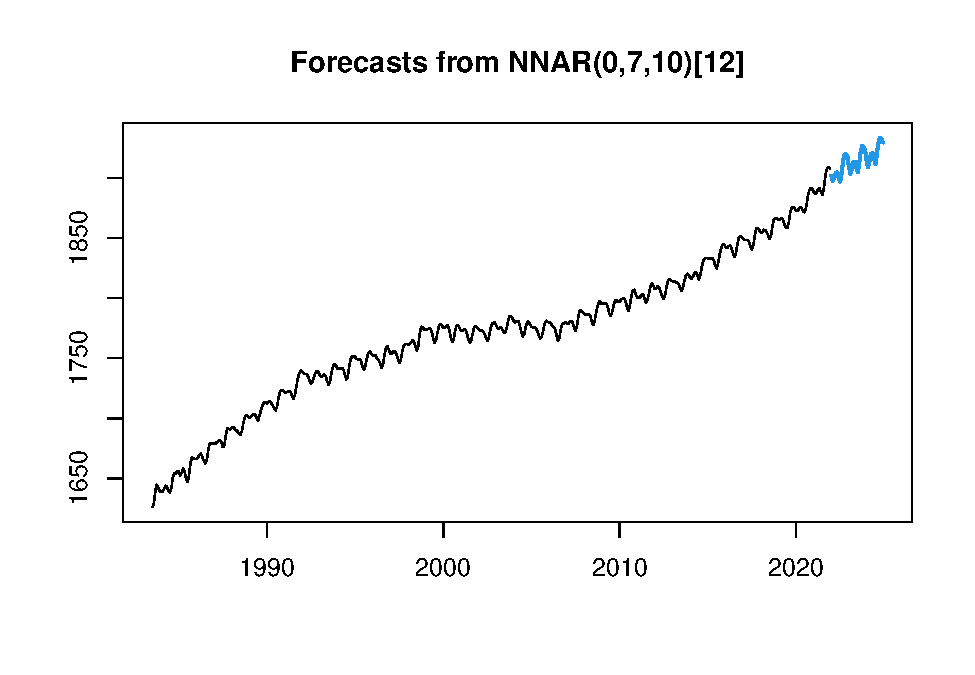
\includegraphics{Methane_Forecasting_files/figure-latex/unnamed-chunk-15-1.pdf}

\subsection{State Space - Smooth}\label{state-space---smooth}

\begin{Shaded}
\begin{Highlighting}[]
\NormalTok{SSES }\OtherTok{\textless{}{-}} \FunctionTok{es}\NormalTok{(methane\_train\_ts,}\AttributeTok{model=}\StringTok{"ZZZ"}\NormalTok{,}\AttributeTok{h=}\DecValTok{36}\NormalTok{,}\AttributeTok{holdout=}\ConstantTok{FALSE}\NormalTok{)}

\NormalTok{SSES\_for }\OtherTok{\textless{}{-}}\FunctionTok{forecast}\NormalTok{(SSES,}\AttributeTok{h=}\DecValTok{36}\NormalTok{, }\AttributeTok{interval=}\StringTok{"prediction"}\NormalTok{)}

\FunctionTok{plot}\NormalTok{(SSES\_for)}
\end{Highlighting}
\end{Shaded}

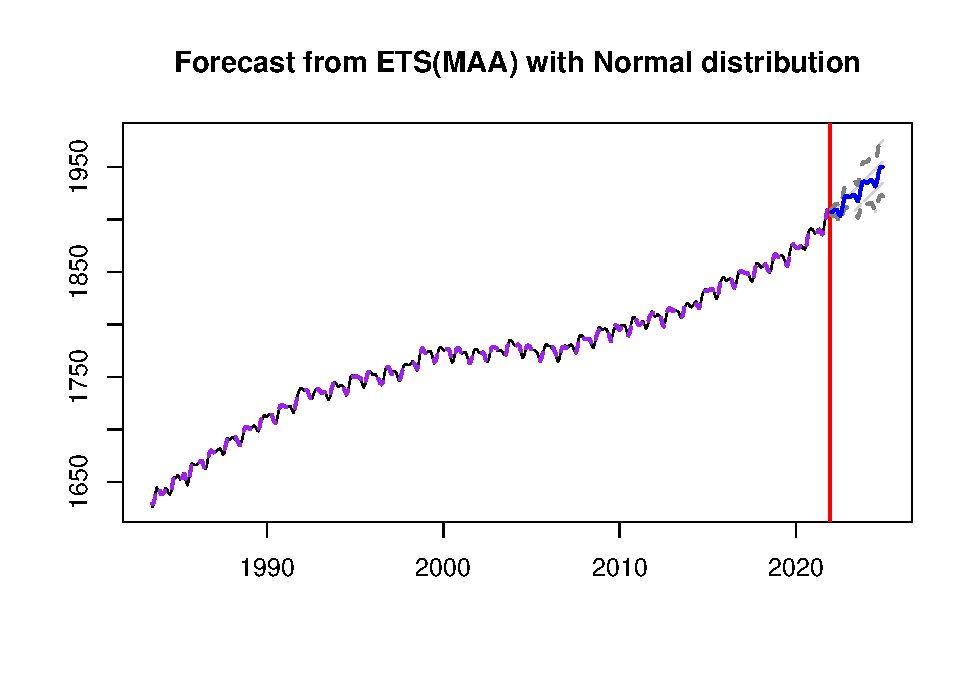
\includegraphics{Methane_Forecasting_files/figure-latex/unnamed-chunk-16-1.pdf}

\begin{Shaded}
\begin{Highlighting}[]
\NormalTok{forecast\_SSES\_accuracy }\OtherTok{\textless{}{-}} \FunctionTok{accuracy}\NormalTok{(SSES}\SpecialCharTok{$}\NormalTok{forecast, methane\_test\_ts)}

\FunctionTok{print}\NormalTok{(forecast\_SSES\_accuracy)}
\end{Highlighting}
\end{Shaded}

\begin{verbatim}
##                 ME     RMSE      MAE        MPE     MAPE      ACF1 Theil's U
## Test set -4.275887 5.649637 4.370569 -0.2219819 0.226947 0.9087947  1.560104
\end{verbatim}

\subsection{State Space - BSM}\label{state-space---bsm}

\begin{Shaded}
\begin{Highlighting}[]
\NormalTok{SSBSM }\OtherTok{\textless{}{-}} \FunctionTok{StructTS}\NormalTok{(methane\_train\_ts,}
                    \AttributeTok{type=}\StringTok{"BSM"}\NormalTok{,}\AttributeTok{fixed=}\FunctionTok{c}\NormalTok{(}\ConstantTok{NA}\NormalTok{,}\ConstantTok{NA}\NormalTok{,}\ConstantTok{NA}\NormalTok{,}\ConstantTok{NA}\NormalTok{))}

\NormalTok{SSBSM\_for }\OtherTok{\textless{}{-}} \FunctionTok{forecast}\NormalTok{(SSBSM,}\AttributeTok{h=}\DecValTok{36}\NormalTok{)}

\FunctionTok{plot}\NormalTok{(SSBSM\_for)}
\end{Highlighting}
\end{Shaded}

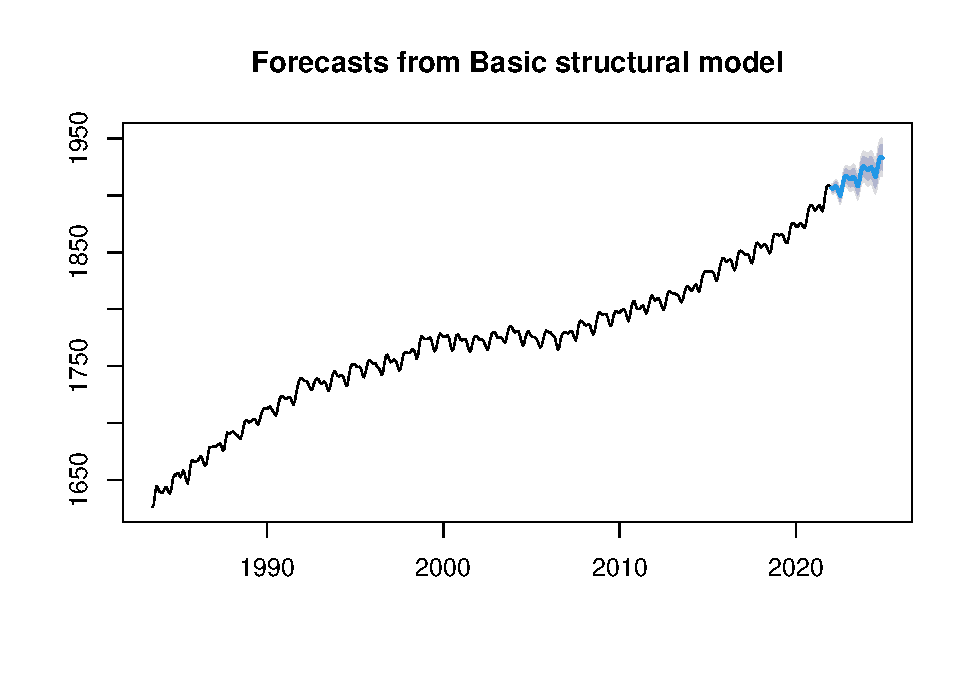
\includegraphics{Methane_Forecasting_files/figure-latex/unnamed-chunk-17-1.pdf}

\begin{Shaded}
\begin{Highlighting}[]
\NormalTok{forecast\_SSBSM\_accuracy }\OtherTok{\textless{}{-}} \FunctionTok{accuracy}\NormalTok{(SSBSM\_for}\SpecialCharTok{$}\NormalTok{mean,methane\_test\_ts)}

\FunctionTok{print}\NormalTok{(forecast\_SSBSM\_accuracy)}
\end{Highlighting}
\end{Shaded}

\begin{verbatim}
##                ME     RMSE      MAE       MPE      MAPE      ACF1 Theil's U
## Test set 4.178408 4.631402 4.196868 0.2171532 0.2181215 0.7558934  1.280794
\end{verbatim}

\section{Performance Comparison}\label{performance-comparison}

\begin{longtable}[]{@{}
  >{\raggedright\arraybackslash}p{(\columnwidth - 12\tabcolsep) * \real{0.4933}}
  >{\raggedleft\arraybackslash}p{(\columnwidth - 12\tabcolsep) * \real{0.0933}}
  >{\raggedleft\arraybackslash}p{(\columnwidth - 12\tabcolsep) * \real{0.0800}}
  >{\raggedleft\arraybackslash}p{(\columnwidth - 12\tabcolsep) * \real{0.0800}}
  >{\raggedleft\arraybackslash}p{(\columnwidth - 12\tabcolsep) * \real{0.0933}}
  >{\raggedleft\arraybackslash}p{(\columnwidth - 12\tabcolsep) * \real{0.0800}}
  >{\raggedleft\arraybackslash}p{(\columnwidth - 12\tabcolsep) * \real{0.0800}}@{}}
\caption{Forecast Accuracy}\tabularnewline
\toprule\noalign{}
\begin{minipage}[b]{\linewidth}\raggedright
\end{minipage} & \begin{minipage}[b]{\linewidth}\raggedleft
ME
\end{minipage} & \begin{minipage}[b]{\linewidth}\raggedleft
RMSE
\end{minipage} & \begin{minipage}[b]{\linewidth}\raggedleft
MAE
\end{minipage} & \begin{minipage}[b]{\linewidth}\raggedleft
MPE
\end{minipage} & \begin{minipage}[b]{\linewidth}\raggedleft
MAPE
\end{minipage} & \begin{minipage}[b]{\linewidth}\raggedleft
ACF1
\end{minipage} \\
\midrule\noalign{}
\endfirsthead
\toprule\noalign{}
\begin{minipage}[b]{\linewidth}\raggedright
\end{minipage} & \begin{minipage}[b]{\linewidth}\raggedleft
ME
\end{minipage} & \begin{minipage}[b]{\linewidth}\raggedleft
RMSE
\end{minipage} & \begin{minipage}[b]{\linewidth}\raggedleft
MAE
\end{minipage} & \begin{minipage}[b]{\linewidth}\raggedleft
MPE
\end{minipage} & \begin{minipage}[b]{\linewidth}\raggedleft
MAPE
\end{minipage} & \begin{minipage}[b]{\linewidth}\raggedleft
ACF1
\end{minipage} \\
\midrule\noalign{}
\endhead
\bottomrule\noalign{}
\endlastfoot
ARIMA & -3.208 & 9.001 & 7.380 & -0.167 & 0.385 & 0.825 \\
SARIMA & 3.086 & 3.331 & 3.086 & 0.161 & 0.161 & 0.629 \\
ARIMA w/ Fourier & -2.914 & 4.346 & 3.320 & -0.151 & 0.172 & 0.895 \\
STL + ETS & -3.916 & 5.274 & 4.073 & -0.203 & 0.212 & 0.907 \\
TBATS & 0.611 & 2.120 & 1.789 & 0.032 & 0.093 & 0.830 \\
Neural Network & 2.611 & 3.624 & 2.702 & 0.136 & 0.140 & 0.705 \\
Neural Network w/ fourier & 7.041 & 8.063 & 7.047 & 0.366 & 0.367 &
0.678 \\
State Space w/ Exponential smoothing & -4.276 & 5.650 & 4.371 & -0.222 &
0.227 & 0.909 \\
State Space w/ BSM & 4.178 & 4.631 & 4.197 & 0.217 & 0.218 & 0.756 \\
\end{longtable}

\section{All Forecasts Plot}\label{all-forecasts-plot}

\begin{Shaded}
\begin{Highlighting}[]
\FunctionTok{autoplot}\NormalTok{(methane\_all\_ts) }\SpecialCharTok{+}
  \FunctionTok{autolayer}\NormalTok{(stl\_ets\_forecast, }\AttributeTok{PI=}\ConstantTok{FALSE}\NormalTok{, }\AttributeTok{series=}\StringTok{"STL+ETS"}\NormalTok{, }\AttributeTok{alpha =} \FloatTok{0.75}\NormalTok{) }\SpecialCharTok{+}
  \FunctionTok{autolayer}\NormalTok{(forecast\_arima, }\AttributeTok{PI=}\ConstantTok{FALSE}\NormalTok{, }\AttributeTok{series=}\StringTok{"ARIMA"}\NormalTok{, }\AttributeTok{alpha =} \FloatTok{0.75}\NormalTok{) }\SpecialCharTok{+}
  \FunctionTok{autolayer}\NormalTok{(forecast\_sarima, }\AttributeTok{PI=}\ConstantTok{FALSE}\NormalTok{, }\AttributeTok{series=}\StringTok{"SARIMA"}\NormalTok{, }\AttributeTok{alpha =} \FloatTok{0.75}\NormalTok{) }\SpecialCharTok{+}
  \FunctionTok{autolayer}\NormalTok{(forecast\_arima\_fourier, }\AttributeTok{PI=}\ConstantTok{FALSE}\NormalTok{, }\AttributeTok{series=}\StringTok{"ARIMA + Fourier"}\NormalTok{, }\AttributeTok{alpha =} \FloatTok{0.75}\NormalTok{) }\SpecialCharTok{+}
  \FunctionTok{autolayer}\NormalTok{(tbats\_forecast,}\AttributeTok{PI=}\ConstantTok{FALSE}\NormalTok{, }\AttributeTok{series=}\StringTok{"TBATS"}\NormalTok{, }\AttributeTok{alpha =} \FloatTok{0.75}\NormalTok{) }\SpecialCharTok{+}
  \FunctionTok{autolayer}\NormalTok{(NN\_for,}\AttributeTok{PI=}\ConstantTok{FALSE}\NormalTok{, }\AttributeTok{series=}\StringTok{"Neural Network"}\NormalTok{, }\AttributeTok{alpha =} \FloatTok{0.75}\NormalTok{) }\SpecialCharTok{+}
  \FunctionTok{autolayer}\NormalTok{(NN\_fourier\_for,}\AttributeTok{PI=}\ConstantTok{FALSE}\NormalTok{, }\AttributeTok{series=}\StringTok{"Neural Network w/ Fourier"}\NormalTok{, }\AttributeTok{alpha =} \FloatTok{0.75}\NormalTok{) }\SpecialCharTok{+}
  \FunctionTok{autolayer}\NormalTok{(SSES\_for,}\AttributeTok{PI=}\ConstantTok{FALSE}\NormalTok{, }\AttributeTok{series=}\StringTok{"State Space w/ Exponential smoothing"}\NormalTok{, }\AttributeTok{alpha =} \FloatTok{0.75}\NormalTok{) }\SpecialCharTok{+}
  \FunctionTok{autolayer}\NormalTok{(SSBSM\_for,}\AttributeTok{PI=}\ConstantTok{FALSE}\NormalTok{, }\AttributeTok{series=}\StringTok{"State Space w/ BSM"}\NormalTok{, }\AttributeTok{alpha =} \FloatTok{0.75}\NormalTok{)}\SpecialCharTok{+}
  \FunctionTok{labs}\NormalTok{(}\AttributeTok{x=}\StringTok{"Time"}\NormalTok{,}
       \AttributeTok{y=}\StringTok{"Methane Concentration (ppb)"}\NormalTok{,}
       \AttributeTok{title =} \StringTok{"Methane Forecasts"}\NormalTok{) }\SpecialCharTok{+}
  \FunctionTok{guides}\NormalTok{(}\AttributeTok{colour=}\FunctionTok{guide\_legend}\NormalTok{(}\AttributeTok{title=}\StringTok{"Forecast"}\NormalTok{))}\SpecialCharTok{+}
  \FunctionTok{xlim}\NormalTok{(}\FunctionTok{c}\NormalTok{(}\DecValTok{2021} \SpecialCharTok{+} \DecValTok{5}\SpecialCharTok{/}\DecValTok{12}\NormalTok{, }\DecValTok{2024} \SpecialCharTok{+} \DecValTok{10}\SpecialCharTok{/}\DecValTok{12}\NormalTok{))}\SpecialCharTok{+}
  \FunctionTok{ylim}\NormalTok{(}\FunctionTok{c}\NormalTok{(}\DecValTok{1875}\NormalTok{,}\DecValTok{1960}\NormalTok{))}
\end{Highlighting}
\end{Shaded}

\includegraphics{Methane_Forecasting_files/figure-latex/unnamed-chunk-20-1.pdf}

\end{document}
